% =====================================================================
%  Extended abstract (3 pages) — City Logistics 2027, Algarve (Portugal)
%  14th International Conference on City Logistics / Institute for City Logistics
%  Candidate for Transportation Research Procedia (Elsevier).
%  NOTE: switch to the official Elsevier "ecrc"/Procedia 3p class when the
%  author guidelines are received; elsarticle used here so it compiles on Overleaf.
% =====================================================================
\documentclass[3p,times]{elsarticle}
\usepackage[utf8]{inputenc}
\usepackage[T1]{fontenc}
\usepackage{graphicx}
\usepackage{booktabs}
\usepackage{hyperref}
\journal{Transportation Research Procedia}

\begin{document}
\begin{frontmatter}

\title{Siting parcel lockers and micro-hubs to decarbonise the last mile:
a data-driven method applied to La Rochelle}

\author[eigsi]{Corwin Fevre}
\author[eigsi]{Tatiana Graindorge}
\author[eigsi]{Robin David}
\author[eigsi]{Jean-Philippe Samier}
\address[eigsi]{EIGSI La Rochelle, 26 rue Vaux de Foletier, 17041 La Rochelle, France}

\begin{abstract}
Automated parcel lockers and micro-hubs are widely promoted to relieve the
externalities of e-commerce last-mile delivery, but their value to the wider
freight system depends less on the technology than on where they are placed. This
paper presents a data-driven method for siting both, and for measuring their
contribution against the current delivery scheme, applied to La Rochelle (France),
a mid-sized ``end-of-line'' city targeting carbon neutrality by 2040. The method
combines a reproducible GIS multicriteria analysis of 148 surveyed collection
points, the public-transport network and population data; a land-compatibility
screen of 95 public car parks; and a transparent emissions model built on
documented factors. An independent demand estimate reproduces the city's
professional freight diagnostic within 8\%, only 23\% of residents live in a
district served by a locker, and 74 car parks are suitable for micro-hub
installation. Diverting home deliveries to well-sited lockers and replacing
in-centre van rounds with hub-and-cargo-bike distribution cut last-mile van
emissions by about half on a real carrier perimeter. For end-of-line cities,
lockers and micro-hubs pay off only when sited together and near demand.
\end{abstract}

\begin{keyword}
city logistics \sep automated parcel lockers \sep micro-hubs \sep last-mile
delivery \sep facility location \sep La Rochelle
\end{keyword}
\end{frontmatter}

\section{Introduction}
E-commerce has pushed business-to-consumer parcel flows into city centres faster
than urban freight systems have adapted, concentrating congestion, emissions,
kerbside conflict and failed deliveries in the streets least able to absorb them.
Automated parcel lockers and micro-hubs are the two levers most cities reach for:
lockers move the final handover out of the home into unattended collection points,
and micro-hubs move the final leg out of the van into cargo-bikes fed from a nearby
consolidation point.

Both levers only work if they are placed well. A locker sited for real-estate
convenience adds an asset without changing flows; one placed where demand,
accessibility and the carrier network coincide restructures rounds. Yet most
siting evidence comes from large metropolises, and mid-sized ``end-of-line''
cities --- peripheral to national corridors and served by few national operators
--- are thinly studied. We address this with a method that sites lockers and
micro-hub land jointly, and that measures their contribution against the current
scheme from open data rather than bespoke assumptions. We apply it to La Rochelle
(about 170,000 inhabitants), whose authority targets carbon neutrality by 2040 and
already restricts city-centre delivery to morning windows with a stated goal of
fully low-emission vehicles.

\section{State of the art and local context}
Locker location is a facility-location problem that balances coverage, demand
density and multimodal accessibility against capital cost and the cannibalisation
of existing collection points [7]. Two solution families dominate the literature:
exact optimisation of locker number, size and location [7], and GIS-based
multicriteria decision-making that ranks candidate sites on accessibility and
demand [9]. Both converge on a compact set of criteria --- proximity to
public-transport nodes and soft modes, residential and footfall density, and
insertion into daily trips --- and report re-delivery cuts near 30\% and lower
per-parcel emissions than van home delivery [6, 8]. A recurring finding is that
lockers are often sited for car rather than transit access, which limits their
reach [8]; transit-anchored pilots such as Valencia and Paris are the corrective
[refs 3--5]. Our method extends this work in two rarely-combined ways: it needs
only openly available data, so it suits mid-sized cities, and it sites lockers
together with the upstream consolidation land that makes them effective.

La Rochelle offers an instructive testbed. A 2018 professional diagnostic based on
the FRETURB model counted about 101,300 goods movements per week across the
agglomeration and 2,290 per day in the historic centre, with e-commerce at 0.31
parcels per household per week --- roughly a fifth of all movements --- concentrated
on a dense historic core and a large social-housing district [ref 1]. The territory
long relied on an electric consolidation centre (2001--2018) and on 72 delivery
bays, four fifths of them undersized. A 2024 study typologised the local logistics
objects, from urban delivery spaces and lockers up to regional gateways, and
described La Rochelle as an end-of-line market with few resident national operators
[ref 2].

\section{Method and data}
The study draws on three EIGSI field projects that form one line of inquiry: a 2021
cargo-bike study of the hyper-centre (633 shops over 38 streets), a 2024 GIS
multicriteria siting of lockers, and the 2025--2026 VerDelivery project on
micro-hub consolidation. From these we assemble a four-step method.
\begin{itemize}\setlength{\itemsep}{1pt}
  \item \emph{Demand.} Weekly e-commerce demand per district is households times
  0.31 parcels/week (FEVAD ratio from the diagnostic).
  \item \emph{Locker siting.} A reproducible GIS workflow (Python/GeoPandas)
  inventories 148 collection points (relays, agencies, nine lockers), adds the
  Y\'elo network (1,414 stops), bike-share and car parks, builds five-minute
  walking buffers, and ranks candidate sites by transit proximity, then
  non-cannibalisation of relays, then demand density.
  \item \emph{Micro-hub land.} A compatibility screen classifies 95 public car
  parks by goods-vehicle access (surface with at least 3 m clearance = candidate;
  below 3 m = conditional; structured = excluded).
  \item \emph{Impact.} Emissions of the current scheme and of each lever are
  computed with documented factors (diesel LGV 0.27 kgCO\textsubscript{2}e/km,
  ADEME; e-cargo-bike 0.013 kgCO\textsubscript{2}e/km; 12 versus 50
  gCO\textsubscript{2} per parcel out-of-home versus home), so every input is
  auditable.
\end{itemize}

\begin{figure*}[t]
  \centering
  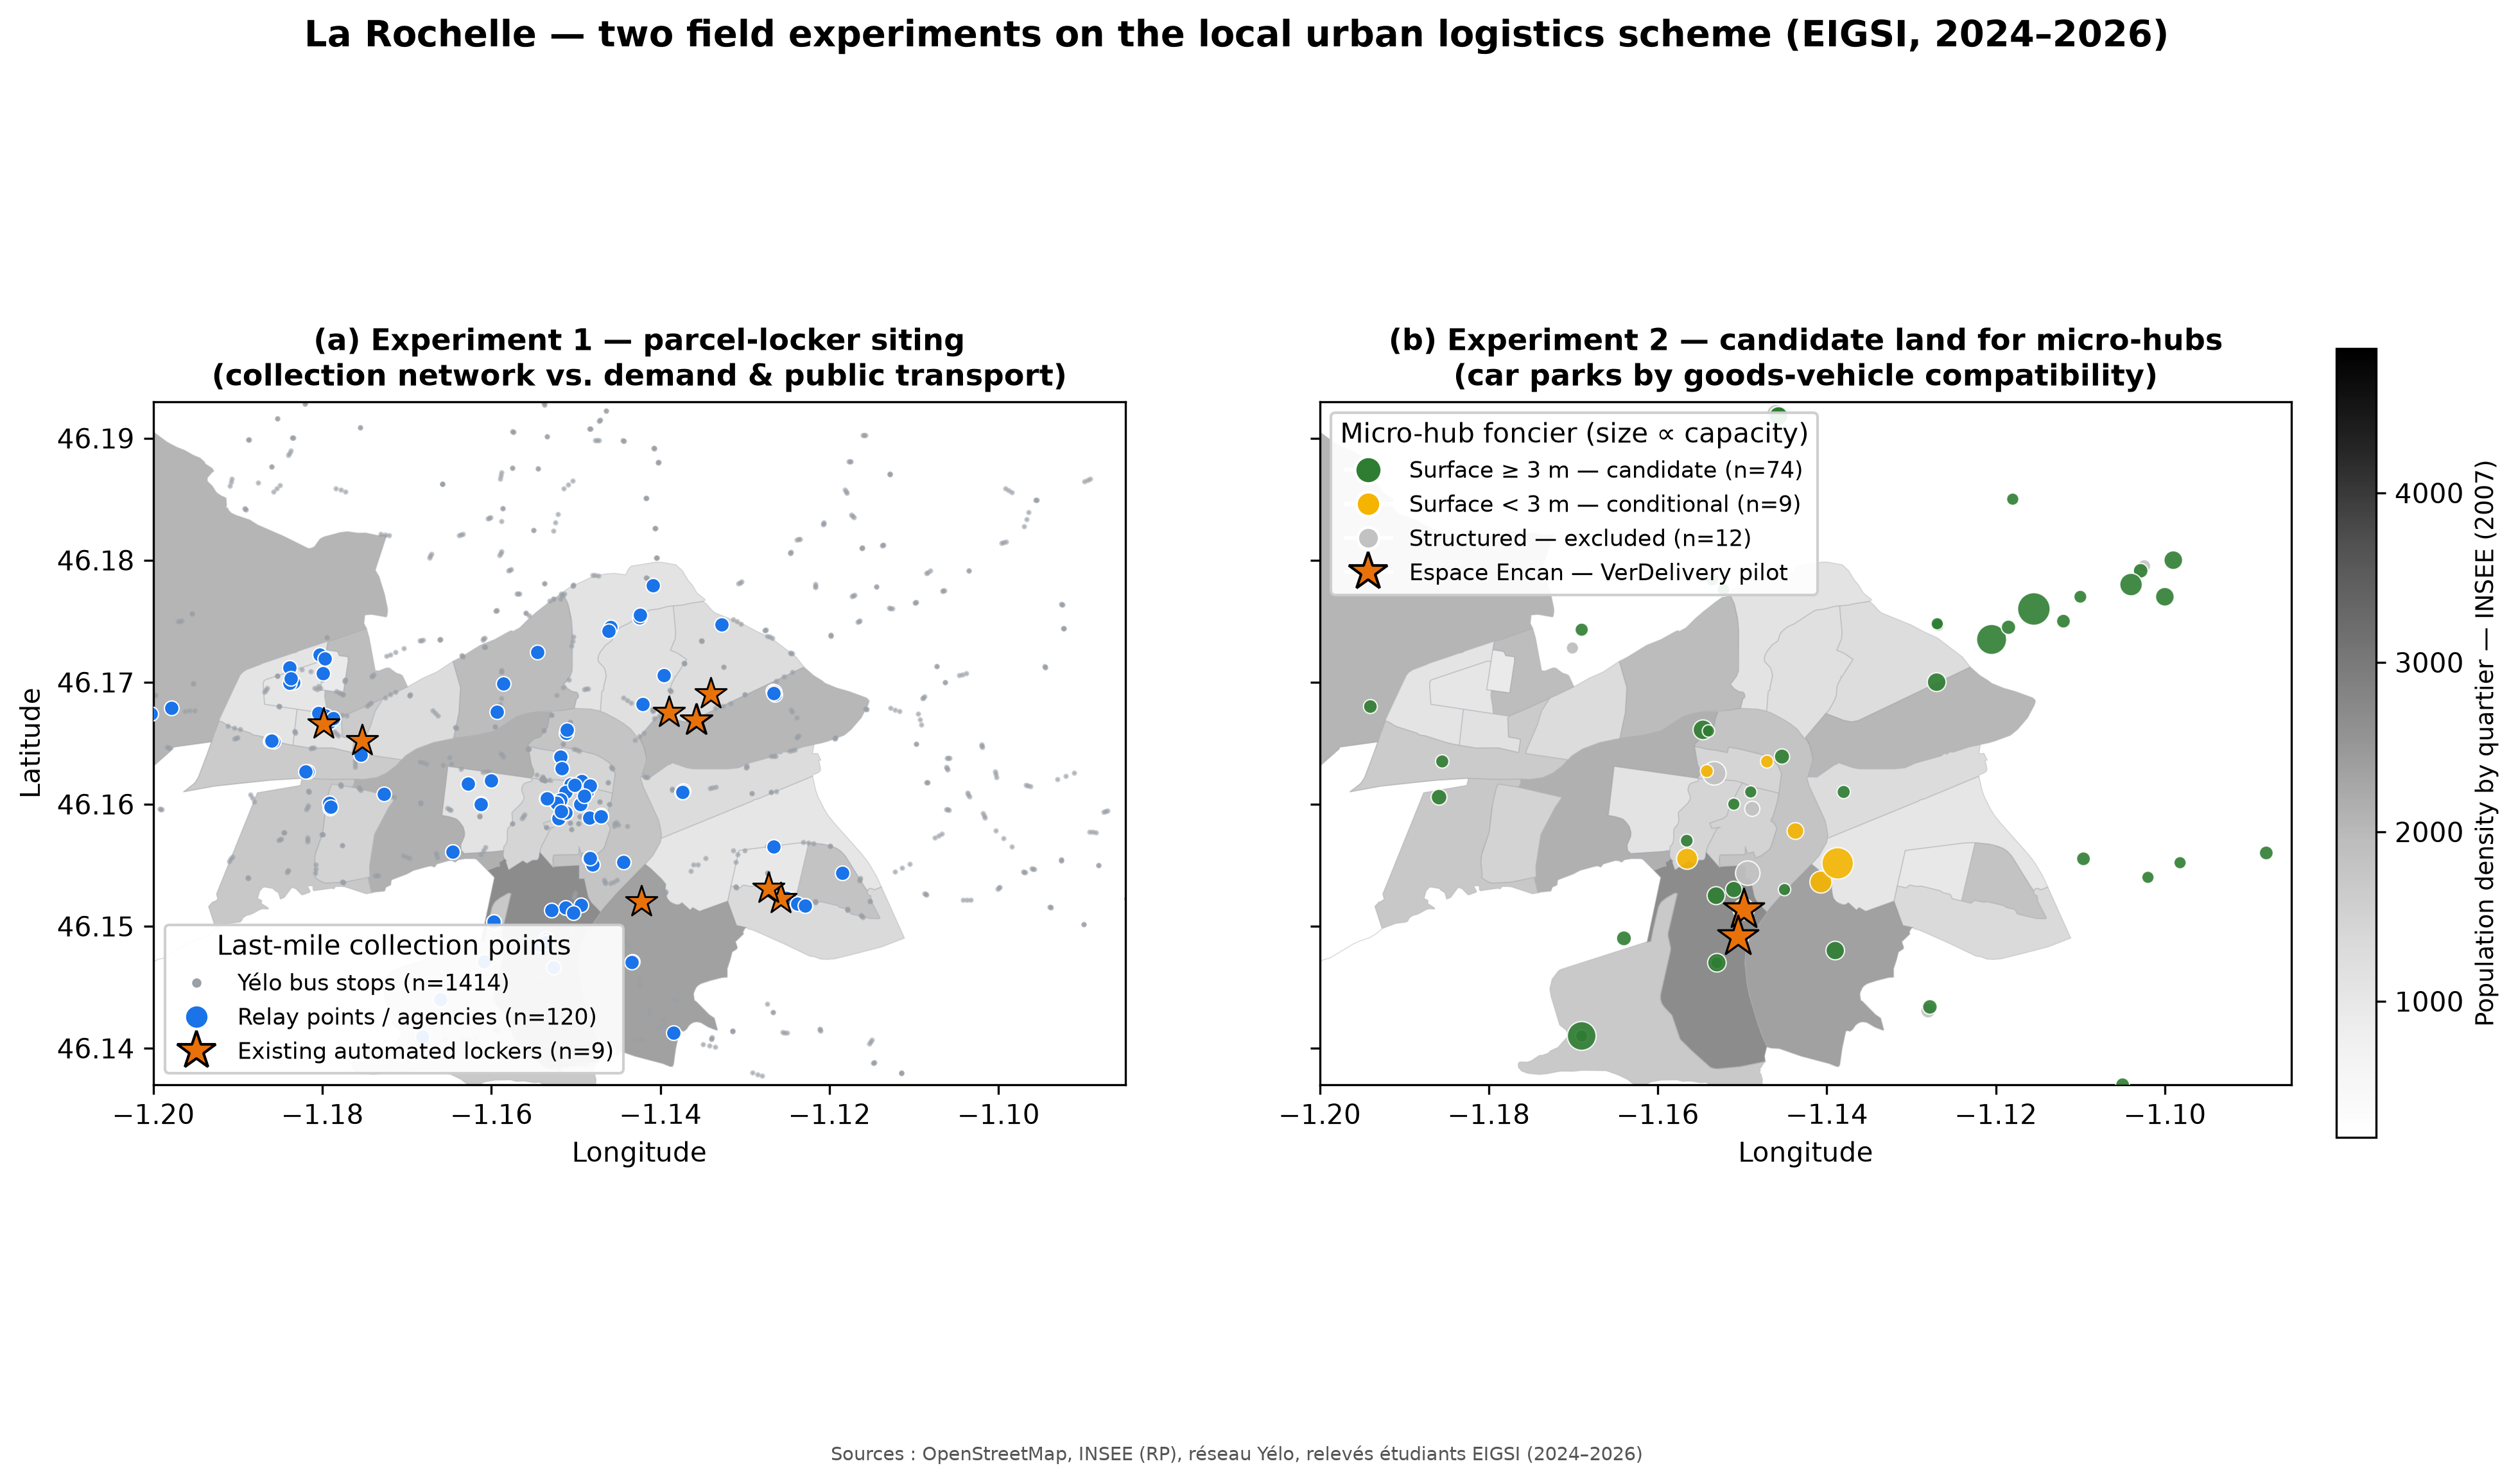
\includegraphics[width=0.98\linewidth]{../../figures/png/larochelle_two_experiments.png}
  \caption{Two field experiments on the local urban logistics scheme of La
  Rochelle, common extent and population backdrop. (a) Locker siting: 120 relay
  points/agencies, 9 existing lockers and the Y\'elo bus network (1{,}414 stops);
  lockers are few and weakly aligned with the densest districts, whereas the
  transit network offers dense candidate anchors. (b) Micro-hub land: 95 car parks
  by goods-vehicle compatibility (74 surface $\geq$ 3 m = candidates, 9 conditional,
  12 excluded; marker size $\propto$ capacity), with the Espace Encan pilot. Field
  data, EIGSI 2024--2026.}
  \label{fig:exp}
\end{figure*}

\section{Results}
The surveyed network reveals a clear supply--demand mismatch (Fig.~\ref{fig:exp}a):
120 relay points but only nine automated lockers, clustered on the centre and the
eastern axis, while the transit network offers 1{,}414 potential anchor nodes
across the demand surface. Our independent demand estimate reproduces the 2018
diagnostic within 8\% --- about 11{,}900 parcels per week --- which validates the
demand model that underpins the impact figures. Despite this, only 23\% of
residents live in a district served by a locker, and several dense districts, among
them Mireuil, Port Neuf and Villeneuve, have none. These become the priority siting
targets, and the multicriteria analysis places ten transit-anchored lockers in
exactly such under-served, high-footfall areas.

The land needed to consolidate flows already exists (Fig.~\ref{fig:exp}b): of 95
public car parks, 74 offer the clearance goods vehicles require, nine are
conditional and twelve are excluded, with the Espace Encan car park anchoring the
pilot. The common objection that mid-sized centres lack space for consolidation
does not hold here.

We measure each lever against the current scheme with documented factors rather
than bespoke numbers. Diverting home deliveries to well-sited lockers saves the
per-parcel difference between home and out-of-home collection: at a fifteen-percent
diversion of the roughly 619,000 parcels handled each year, about 3.5 tonnes of
CO\textsubscript{2} annually, plus a further 0.7 tonnes from fewer failed
re-deliveries, a figure that scales with coverage and adoption. On a real carrier
perimeter of three vans, replacing in-centre rounds with depot-to-hub stems plus
cargo-bike distribution cuts last-mile van emissions from about 16 to 8.5 tonnes of
CO\textsubscript{2} per year, a reduction near one half. Because the cargo-bike
factor is some twenty times smaller than the van's, this saving is driven by the
van-kilometres removed and is robust to the cargo-bike assumption; the remaining
sensitivity lies in the tour lengths, which the model exposes as inputs to be
measured from real traces.

\section{Discussion}
Siting is the decisive lever. Transit-anchored, demand-aware placement maximises
use and modal-shift potential, whereas sites chosen for availability alone risk
cannibalising relay points, which supply about a third of a host shop's turnover,
without net gain. Real barriers remain, from a durable preference for home delivery
and thin network density to installation cost, accessibility for people with
reduced mobility, and governance. The lesson for end-of-line cities is integration:
with few resident national operators, a locker network returns system benefits only
when it is co-designed with consolidation and local cyclo-logistics. Since the
compatible land already exists, the binding constraint is institutional rather than
spatial.

\section{Conclusion}
The study contributes a low-data, reproducible method that sites parcel lockers and
micro-hub land together and measures their contribution against the current scheme
from open data and documented factors. Applied to La Rochelle, it validates the
demand model against an independent source, exposes a coverage gap that motivates
siting, and shows that combining well-sited lockers with hub-and-cargo-bike
consolidation roughly halves last-mile van emissions on a real perimeter. Future
work will measure real tour lengths and adoption, add a capacitated coverage
optimisation of the candidate sites [7], and feed the results into the
agglomeration's logistics roadmap.

\section*{Statements}
\noindent\footnotesize\textbf{Data availability.} La Rochelle figures derive from
the corpus (refs 1--5); datasets, figure scripts and the impact model are available
from the authors. \textbf{Author contributions (CRediT).} Conceptualisation
T.~Graindorge, C.~Fevre; data/software R.~David, C.~Fevre; analysis all; draft
C.~Fevre; supervision T.~Graindorge, J.-P.~Samier (to be confirmed).
\textbf{AI-usage disclosure.} Drafting/editing were AI-assisted under author
supervision; all data, analysis and conclusions are the authors' own.
\textbf{Conflicts of interest.} None.
\normalsize

\section*{References}
{\footnotesize
\begin{enumerate}\setlength{\itemsep}{0pt}
\item Interface Transport (2018). \emph{Base de connaissances marchandises --- CdA de La Rochelle.} [corpus]
\item Interface Transport (2024). \emph{\'Etude sur les besoins en foncier logistique --- CdA de La Rochelle.} [corpus]
\item EIGSI (2021). \emph{Projet I\&E n\textdegree1 --- Cargo-V\'elo La Rochelle.} [corpus]
\item EIGSI (2024). \emph{Projet IE 49 --- LOG\_URB\_ROCHELLE (lockers \& micro-hubs).} [corpus]
\item EIGSI (2025--2026). \emph{Projet PIE 26-38 --- VerDelivery.} [corpus]
\item Iwan, S., Kijewska, K., Lemke, J. (2016). Analysis of parcel lockers' efficiency as the last-mile delivery solution --- the results of the research in Poland. \emph{Transportation Research Procedia} 12, 644--655. \texttt{doi:10.1016/j.trpro.2016.02.018}
\item Deutsch, Y., Golany, B. (2018). A parcel locker network as a solution to the logistics last-mile problem. \emph{Int.\ J.\ of Production Research} 56(1--2), 251--261. \texttt{doi:10.1080/00207543.2017.1395490}
\item Lachapelle, U., Burke, M., Brotherton, A., Leung, A. (2018). Parcel locker systems in a car-dominant city. \emph{Journal of Transport Geography} 71, 1--14. \texttt{doi:10.1016/j.jtrangeo.2018.06.022}
\item Bovkir, R., Moslem, S., Pilla, F. (2025). GIS-based fuzzy multi-criteria decision-making for selecting optimal parcel lockers location: a case study in Dublin, Ireland. \emph{Land Use Policy} 158, 107771. \texttt{doi:10.1016/j.landusepol.2025.107771}
\end{enumerate}}

\end{document}
